%%%%%%%%%%%%%%%%%%%%%%%%%%%%%%%%%%%%%%%%%%%%%%%%%
% Documento Principal Geometria Analítica
% Gersonilo Oliveira da Silva
%%%%%%%%%%%%%%%%%%%%%%%%%%%%%%%%%%%%%%%%%%%%%%%%%

    \documentclass [a4paper,12pt,brazil]{book}
    \usepackage[utf8]{inputenc}
    \usepackage{multicol}
    \usepackage[brazil]{babel}
    \usepackage{amssymb,amscd,latexsym}
    \usepackage{amsmath}
    \usepackage{color}
    \usepackage{epsfig}
    %\usepackage[dvips]{graphicx}
    %\usepackage{srcltx}

    \setlength{\oddsidemargin}{0.46cm}
    \setlength{\textwidth}{15cm}
    \setlength{\topmargin}{-0.79cm}
    \setlength{\headheight}{0.75cm}
    \setlength{\headsep}{0.50cm}
    \setlength{\textheight}{24cm}
    \setlength{\parindent}{1.0cm}
    \renewcommand{\baselinestretch}{1.1}
    \pagenumbering{arabic} \setcounter{page}{6}
%    \setlength{\parskip}{0.2 cm}

%    \newtheorem {teorema}{Teorema}[chapter]
%    \newtheorem {proposicao}[teorema]{Proposição}
%    \newtheorem {lema}[teorema]{Lema}
%    \newtheorem {definicao}[teorema]{Definição}

    \newcommand {\cqd}{\hfill $\blacksquare$ \vspace{0.5cm}}

    \pagestyle{headings}
    \newtheorem{theorem}{Teorema}[chapter]
    \newtheorem{acknowledgement}[theorem]{Acknowledgement}
    \newtheorem{algorithm}[theorem]{Afirmação}
    \newtheorem{axiom}[theorem]{Axioma}
    \newtheorem{case}[theorem]{Case}
    \newtheorem{claim}[theorem]{Claim}
    \newtheorem{conclusion}[theorem]{Conclusion}
    \newtheorem{condition}[theorem]{Condition}
    \newtheorem{conjecture}[theorem]{Conjectura}
    \newtheorem{corollary}[theorem]{Corolário}
    \newtheorem{criterion}[theorem]{Criterion}
    \newtheorem{definition}[theorem]{Definição}
    \newtheorem{example}{Exemplo}
    \newtheorem{exercise}[theorem]{Exercício}
    \newtheorem{lemma}{Lema}[chapter]
    \newtheorem{notation}[theorem]{Notation}
    \newtheorem{problem}[theorem]{Problem}
    \newtheorem{proposition}[theorem]{Proposição}
    \newtheorem{remark}{Observação}[chapter]
    \newtheorem{solution}[theorem]{Solution}
    \newtheorem{summary}[theorem]{Summary}
    \newenvironment{proof}[1][\textbf{Demonstração:}\hspace{0.2cm}]{\textit{#1}}{\begin{flushright}\itshape{QED.}\end{flushright}}


%\includeonly{ApendiceA}


\begin{document}

\pagestyle{headings}

%%%%%%%%%%%%%%%%%%%%%%%%%%%%%%%%%%%%%%%%%%%%%%%%%
% Relatório Final - Projeto de Pesquisa
%Métodos de Otimização
% Baltz & Machado
% Capa
%%%%%%%%%%%%%%%%%%%%%%%%%%%%%%%%%%%%%%%%%%%%%%%%%


\thispagestyle{empty}


\begin{center}
{\huge \textbf{Ministério da Educação}} \\
{\huge \textbf{Universidade Federal do Agreste de Pernambuco}}
\end{center}

\vspace {8cm}

\begin{center}
{\huge \textbf{Relatório Final}} \\
{\huge \textbf{Métodos de Otimização}}
\end{center}



%%%%%%%%%%%%%%%%%%%%%%%%%%%%%%%%%%%%%%%%%%%%%%%%%%%%%%%%%%%%%%%%%%%%%%%%%%%%%%%%%%%%%%%%%%%%%%%%%%%%%%%%%%%%%%%%%%%%%%%%%%%%%%%%%%%%%%%%%%%%%%%

\newpage

\thispagestyle{empty}

\begin{center}
$\propto$
\end{center}


%%%%%%%%%%%%%%%%%%%%%%%%%%%%%%%%%%%%%%%%%%%%%%%%%%%%%%%%%%%%%%%%%%%%%%%%%%%%%%%%%%%%%%%%%%%%%%%%%%%%%%%%%%%%%%%%%%%%%%%%%%%%%%%%%%%%%%%%%%%%%%%


\newpage

\thispagestyle{empty}



\begin{center}
{\huge \textbf{Ministério da Educação}} \\
{\huge \textbf{Universidade Federal do Agreste de Pernambuco}}
\end{center}

\vspace{6cm}

\begin{center}
{\huge \textbf{Relatório Final}} \\
{\huge \textbf{Métodos de Otimização}}
\end{center}

\vspace{5cm}

\begin{center}
{\Large\textit{Baltz}}\\
{\Large\textit{Machado}}\\
{\Large\textit{Gersonilo Oliveira da Silva}}
\end{center}


\newpage 


%\thispagestyle{empty}
%
%\begin{center}
%$\propto$
%\end{center}
%
%\vspace{10cm}
%
%
%\begin{array}{c}
%
%\textbf{Dados \hspace{0.2cm} Internacionais \hspace{0.2cm} de \hspace{0.2cm} Catalogação \hspace{0.2cm} da \hspace{0.2cm} Fonte.} \\
%
%\begin{tabular}{|c| p{8cm} | p{8cm}}
%\hline
%
%\begin{flushleft}
%B897a  \hspace{1cm} Gersonilo Oliveira da Silva
%\end{flushleft}
%\\
     %\hspace{1.5cm}		Geometria Analítica. Gersonilo Oliveira da Silva. 1º edição. Garanhuns. 2020.\\\\\\
							%
		 %
		 %\begin{flushleft}
		 %ISBN 1234566788-999
		 %\end{flushleft}
			%\\\\\\
										%
		%
			%\hspace{0.8cm} 1. Matemática 2. Álgebra Linear I. Título	\\\\
				
				                                           
																									
																						%\hspace{4cm} CDD 9999999 \\
				                                            %
																						%\hspace{4cm} CDU 9999999-999 \\
%
%\hline
%
%\end{tabular}
%
%\end{array}

\newpage 


\thispagestyle{empty}

\begin{center}
$\propto$
\end{center}

\newpage 


\thispagestyle{empty}

\begin{center}
$\propto$
\end{center}
\renewcommand{\baselinestretch}{1.0} \thispagestyle{plain}\pagenumbering{arabic} \tableofcontents
%%%%%%%%%%%%%%%%%%%%%%%%%%%%%%%%%%%%%%%%%%%%%%%%%
% Relatório Final - Projeto de Pesquisa
% Métodos de Otimização
% Baltz & Machado
% Introdução
% %%%%%%%%%%%%%%%%%%%%%%%%%%%%%%%%%%%%%%%%%%%%%%%%%

%\pagenumbering{arabic} \setcounter{page}{6} \thispagestyle{empty}
\addcontentsline{toc}{section}{{\bf Introdução}}
\chapter*{\textbf{\LARGE{Introdução}}}


\vspace{2cm}

\begin{center}
\textit{Para Tales, a questão primordial não era o que sabemos,\\ mas como o sabemos.}
\end{center}

\begin{flushright}
\textsl{Aristóteles}
\end{flushright}

\begin{center}
\textit{Evita o que o pertuba a mente e o que a alma esmaga,\\ Aprimora a razão, esmera os valores teus;\\ E transpondo, enfim, a prefulgante plaga\\
Tu, entre os imortais, serás também um deus.}
\end{center}

\begin{flushright}
\textsl{Pitágoras}
\end{flushright}

\begin{center}
\textit{Não posso me convencer de que, quando se soma uma a um, o um a que foi\\
feita a adição se transforma em dois, ou que duas unidades somadas farão\\ dois em consequência da adição. Não posso entender como quando\\
separadas cada uma era uma e não dois e agora, quando reunidas, a\\ simples justaposição ou encontro delas seja causa de se tornarem dois.}
\end{center}

\begin{flushright}
\textsl{Diálogo de Platão}
\end{flushright}

\begin{center}
\textit{É, pois, sem razão, que os geômetras são acusados de ensinarem apenas\\ quimeras e de não terem na sua ciência nada de bom e de belo. Eu, pelo\\ contrário, sustento que eles, sem disso fazerem ostentação, ensinam coisas\\ que são, ao mesmo tempo, muito boas e muito belas. Pois toda bondade e\\ toda beleza não resulta, forçosamente, da ordem e da proporção? Ora, de\\ que coisas se ocupa o geômetra, senão da ordem e da porporção?}
\end{center}

\begin{flushright}
\textsl{Aristóteles - Tratado de Filosofia}
\end{flushright}

\begin{center}
\textit{Ptolomeu uma vez perguntou se havia um caminho mais curto para a\\ geometria que o estudo de Os elementos e Euclides lhe respondeu que não\\ havia estrada real para a geometria.}
\end{center}

\begin{flushright}
Proclus Diadocus
\end{flushright}


%\par Aqui fazemos uma análise geométrica dos instrumentos matemáticos modernos a fim de expor em linha reta o que se faz necessário ao conhecimento de um Bacharel em Ciência da Computação. Em nosso primeiro capítulo discorremos sobre os efeitos históricos do desenvolvimento da Geometria partindo de sua origem, sendo esta considerada literariamente, em Os elementos de Euclides, partindo para o descorrer da origem das coordenadas na geometria, feita por Descartes. Depois partimos para a descrição sucinta da teoria das matrizes no segundo capítulo. Feita muito respaldada na ementa do curso. Seguindo com a geometria propriamente dita. Considerando os espaços $\mathbb{R}^2$ e $\mathbb{R}^{3}$ seus elementos e suas propriedades. Depois vemos as curvas provindas das seções cônicas, e por conseguinte as superfíceis quadrádicas. Findando deste modo o propósito deste compêndio.

%%%%%%%%%%%%%%%%%%%%%%%%%%%%%%%%%%%%%%%%%%%%%%%%%
% Relatório Final - Projeto de Pesquisa
% Métodos de Otimização
% Baltz & Machado
% Capítulo 1
%%%%%%%%%%%%%%%%%%%%%%%%%%%%%%%%%%%%%%%%%%%%%%%%%


\chapter{\Large{Métodos Matemáticos de Otimização}}\label{chp:1}


\section{{O Conceito de Otimização}}

\hspace{0.8cm}
Diz-se otimização, o processo que tem como objetivo encontrar condições que
minimizam ou maximizam algo (seja energia, tempo, dinheiro, etc). Sendo este,
muitas vezes um trabalho árduo, custoso.

Dessa maneira, na matemática, tal processo é amplamente utilizado quando
busca-se valores em conjunto \textit{A} (que pode terrestrições), com o
objetivo de encontrar uma solução ótima (a melhor resposta para o problema),
aplicando os valores de \textit{A} em numa função objetivo predefinida.

Podendo assim, ser representada da seguinte forma:

    Dada a função
        \begin{equation}
            f : A \rightarrow \mathbb{R}
        \end{equation}

        \begin{itemize}
                \item Maximização pode ser definida como:
        \end{itemize}

                busca pelo elemento \(x_0 \in A\), que satisfaz:

                    \begin{equation}
                        f(x_0) \geq f(x);
                    \end{equation}

                para todo \(x \in A\).

        \begin{itemize}
                \item Minimização pode ser definida como:
        \end{itemize}

                busca pelo elemento \(x_0 \in A\), que satisfaz:

                    \begin{equation}
                        f(x_0) \leq f(x);
                    \end{equation}

                para todo \(x \in A\).

\vspace{\baselineskip}
Com isso, podemos agora entender como esse processo pode ser custoso. Iniciando
com fato de que existem os pontos máximos e mínimos (pontos críticos), locais
e globais, no espaço das funções. Sendo os pontos críticos locais, aqueles que
não são os menores ou maiores valores para a minimização e maximização,
respectivamente. E os pontos globais, aqueles que representam o menor ou maior
valor no espaço das funções, para a minimização e maximização, respectivamente.

Criando assim, uma certa incerteza ao encontrar um valor crítico numa função,
já que é estritamente difícil saber se o ponto crítico encontrado é local ou
global. Como pode-se perceber na Figura
\ref{grafico_local_global_pontosCriticos}.


\begin{figure}[h]
    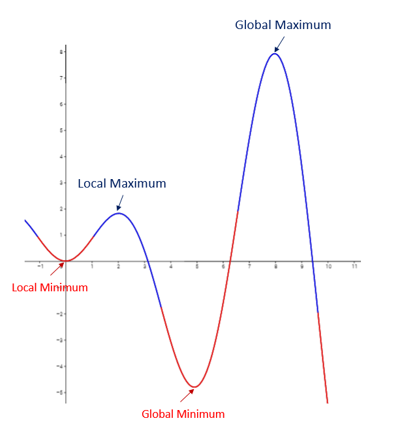
\includegraphics[width=0.43\textwidth]
        {src/grafico_local_global_pontosCriticos.png}
    \centering
    \caption{Exemplo de pontos críticos locais e globais indicados no gráfico
        de uma função}
    \label{grafico_local_global_pontosCriticos}
\end{figure}

Como na grande maioria dos casos não é possível conhecer antecipadamente todo
o espaço gerado pela função, a busca pelo ótimo pode resultar em pontos
críticos locais. Donde, dependendo do problema tais resultados chegam a ser
satisfatórios. No entanto, quando o objetivo é estritamente encontrar os máximos
ou mínimos globais, o trabalho necessário acaba sendo mais custoso, pelo fato de
que há a incerteza da existência de mais pontos na grande maioria dos problemas.

Ademais, o conjunto $A$, no qual contém os valores aplicáveis no problema, podem
respeitar restrições, fazendo com que o campo de respostas do problema, não seja
contínuo.

\section{{Otimização de Funções à Uma Variável Real}}

\hspace{0.8cm}

Evidente que funções possuem as variáveis dependentes (a qual representa o
objeto da otimização) e variáveis independentes (cujo suas grandezas podem ser
selecionadas), podemos denotar que, para a equação

\begin{equation}
	y = f(x),
\end{equation}
quando buscamos otimizá-la, temos como objetivo encontrar valores que quando
aplicados à \textit{x}, temos o mínimo ou máximo valor \textit{y} (seja ele
local, ou preferencialmente global).

Partindo dessa perspectiva, acaba surgindo a necessidade de utilizar algum
recurso para encontrar os pontos críticos. E nesse sentindo, pode-se utilizar
a técnica de \textbf{derivação}, donde, oferece como recurso a possibilidade de
identificar tais pontos.

A derivada é a representação da taxa de variação de uma função, em relação a
um ponto. A partir daí, podemos observar um fator interessante; por exemplo,
quando a função está num ponto máximo, existem duas possibilidades, a primeira,
sendo a função parando de crescer e em seguinda se tornando indefinida; e a
segunda possibilidade quando a função para de crescer e começa a decrescer.
Com isso, é importante ressaltar que por definição, quando a derivada (taxa de
variação) em um ponto é positiva, a função cresce, e quando negativa a função
decresce. Conclui-se que, quando a taxa de variação é zero, a função ou para de
crescer ou de decrescer, sendo assim um ponto de máximo ou de mínimo.

Com o uso da derivada, podemos pensar num método de otimização bastante simples,
considerando \(f(x)\) a função que queremos otimizar e \(f'(x)\) sua função
derivada, podemos dizer que o conjunto $O$ possui todos os ótimos locais e
globais de \(f(x)\):

\begin{equation}
    O := \{f(x) | f'(x) = 0\}
\end{equation}


Portanto, aplicando um filtro em $O$ para obeter o máximo e mínimo do conjunto,
acabamos por obeter o máximo e mínimo de \(f(x)\):


\begin{equation}
    max(f(x)) = max(O)
\end{equation}

\begin{equation}
    min(f(x)) = min(O)
\end{equation}


Então podemos perceber dois problemas; determinar como encontrar os pontos onde
a derivada se anule, e determinar se temos de fato todos os pontos.

Considerando por agora, apenas o problema de encontrar os pontos críticos;

Entendendo melhor, a taxa de variação de uma função \(y=f(x)\) em relação a
\(x\), é dada pela relação \(\Delta y / \Delta x\). Sendo esse resultado
correspondente a tangente do ângulo formado pela intersecção entre a reta e a
curva da função \(y\); o coeficiênte ângular da reta à curva.

Sendo o cálculo da taxa de variação demonstrado pela Figura
\ref{derivada_padrao}.

\begin{figure}[h]
    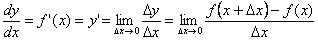
\includegraphics[width=0.45\textwidth]
        {src/derivada_padrao.jpg}
    \centering
    \caption{Derivada: taxa de variação \(dy/dx\).}
    \label{derivada_padrao}
\end{figure}

Partindo desse princípio, é intríseco saber que uma função pode ser derivada
mais de uma vez, sendo essas derivadas, denominadas de `primeira derivada',
`segunda derivada' e por ai em diante. De modo que, a segunda derivada é
a taxa de variação da primeira derivada. Concluindo-se que dada a função
\(f(x)\), sua primeira derivada é \(df/dx = p(x)\), e sua segunda derivada
\(dp/dx = s(x)\).

Considerando que a primeira e segunda derivada são as comumente utilizadas,
pode-se agora entender a relação entre elas e a função original.

Já sabido que a primeira derivada representa a taxa de variação de um ponto na
curva, a segunda derivada proporciona informações complementares, como por
exemplo, se é um ponto de máximo, mínimo ou inflexão, de modo que ela determina
a concavidade da curva naquele ponto. Como pode-se ver na Figura
\ref{relacao_primeira_segunda_derivada}. E de modo construtivo, é importante
ressaltar que é importante o estudo do gráfico das derivadas de uma função.

\begin{figure}[h]
    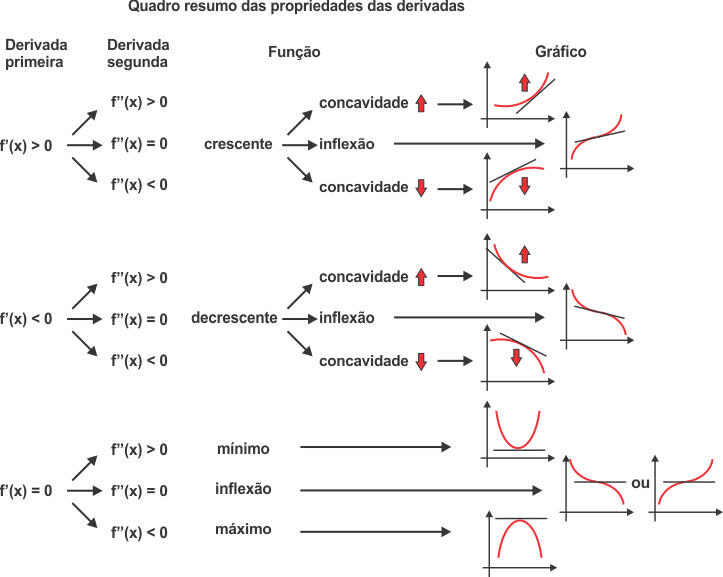
\includegraphics[width=0.65\textwidth]
        {src/relacao_primeira_segunda_derivada.jpg}
    \centering
    \caption{Propriedades e relação da primeira e segunda derivada.}
    \label{relacao_primeira_segunda_derivada}
\end{figure}


\section{{Programando o Método}}

\hspace{0.8cm}


A própria definição da derivada já nos oferece uma uma visão simples de como
ela pode ser implementada num programa de computador. Mas com alguns nuances
que devem ser levados em consideração. Segue a tal implementação:

\begin{lstlisting}[]

pub fn derive1x1_v1<F>(f: &F, x: f64) -> f64
where
    F: Fn(f64) -> f64,
{
    (f(x + h) - f(x)) / h
}


\end{lstlisting}


Essa implementação é ingenua no que se diz respeito a precisão da operação. O
uso depende da aplicação, caso se queira prezar por velocidade de calculo e 
muito pouco sobre precisão, talvez essa solução seja boa o suficiente. O
problema com com precisão desta implementação é que não se é levado em
consideração o aspecto infinitesimal da variação (\(\Delta X\) na figura 1.2, ou
a variável h na implementação em Rust), já que é por este aspecto que
definimos a derivada. Não temos como ter uma variável com tal propriedade num
programa de computador. Como consequência, \(f(x + h) - f(x)\) já é calculada
de forma falha, entregando uma variação diferente da que seria quando se tem
uma variável infinitesimal. O que de fato é entregue é a variação um pouco mais
a frente do ponto esperado.

A partir dai podemos reformular considerando esse deslocamento, redefinindo
da seguinte forma:


\begin{equation}
    f'(x) = \frac{f(x + h) - f(x - h)}{2h}
\end{equation}

Que é equivalente à:

\begin{equation}
    f'(x) = \frac{f(x + h) - f(x - h)}{(x + h) - (x - h)}
\end{equation}


Usaremos essa segunda formulação por motivos de custo de multiplicação de de
números reais se comparado a somas e subtrações, além da possível perca de
precisão. Assim conseguimos compensar o tal deslocamento numa nova função
insignificantemente mais custosa e mais precisa:


\begin{lstlisting}[]

pub fn derive1x1_v2<F>(f: &F, x: f64) -> f64
where
    F: Fn(f64) -> f64,
{
    let x1 = x - h;
    let x2 = x + h;

    let y1 = f(x1);
    let y2 = f(x2);
    return (y2 - y1) / (x2 - x1);
}


\end{lstlisting}






\textcolor[rgb]{1,0,0}{\section{{Otimização de Funções à Várias Variáveis}}}

\hspace{0.8cm}





%

%%%%%%%%%%%%%%%%%%%%%%%%%%%%%%%%%%%%%%%%%%%%%%%%%
% Relatório Final - Projeto de Pesquisa
% Métodos de Otimização
% Baltz & Machado
% Capítulo 2
%%%%%%%%%%%%%%%%%%%%%%%%%%%%%%%%%%%%%%%%%%%%%%%%%


\chapter{\Large{Métodos Clássicos de Otimização}}\label{chp:2}


\section{{O Método de Newton}}


\subsection{Entendendo o Método}

%TODO: Falar de funções bem definidas

\hspace{0.8cm}
O Método de Newton, foi desenvolvido com o objetivo de encontrar estimativas
para as raízes de uma função. De modo que, a execução do método é feita de
forma iterativa, repetindo sempre o mesmo processo, atualizando o mesmo valor.

Este método faz uso do recurso de derivação, existindo, uma relação muito
forte com o ângulo da reta tangente ao ponto, na função. Ademais, é
importante ressaltar, que é necessário um palpite inicial, que represente
o valor de \textit{x}, no qual, partindo desse valor, será buscado a raiz.
E com isso, vamos entender como o dado método funciona.

Partindo do princípio do método, o objetivo, será utilizar a reta tangente a um
ponto, para gerar valores cada vez mais próximos da raiz daquela função. De
modo que, será analisado a interseção da reta tangente com o eixo das
abscissas. E sendo, a diferença do valor x da entrada da função com o valor da
fração entre a função e sua derivada no mesmo ponto, o novo valor de entrada na
função, construindo assim várias iterações, gerando valores cada vez mais
próximos da raiz. Como será visto, a seguir:

Já sabido que a equação da reta é dada como:

\begin{equation}
    (y - y_0) = m(x - x_0).
\end{equation}

E levando em conta que temos como objetivo encontrar $x$, que é um ponto
sobreposto no eixo x, podemos considerar $y=0$, logo:

\begin{equation}
    -y_0=m(x-x_0).
\end{equation}

Com isso, sabemos que $y_0$ é a imagem da função $f(x_0)$, e $m$ representa o
ângulo da reta tangente ao ponto $x_0$, ou seja: $m=f'(x_0)$. Desenvolvendo
essa equação, temos:

\begin{equation}
    -f(x_0) = f'(x_0)(x-x_0),
\end{equation}

\begin{equation}
    -f(x_0) = f'(x_0)x - f'(x_0)x_0,
\end{equation}

\begin{equation}
    0 = f'(x_0)x - f'(x_0)x_0+f(x_0),
\end{equation}

\begin{equation}
    0 = x - x_0 + \frac{f(x_0)}{f'(x_0)},
\end{equation}

\begin{equation}
    x = x_0 - \frac {f(x_0)}{f'(x_0)}.
\end{equation}\\

E com isso, exemplificando em um gráfico, temos que, sendo $f(x)=-x^2+2x$, o
palpite inicial $x_0=1.5$, $P1$ sendo o ponto que representa $x_0$ aplicado
a função $f$ e $x1$ a interseção da reta tangente à $P1$ com o eixo x.

\begin{figure}[ht]
    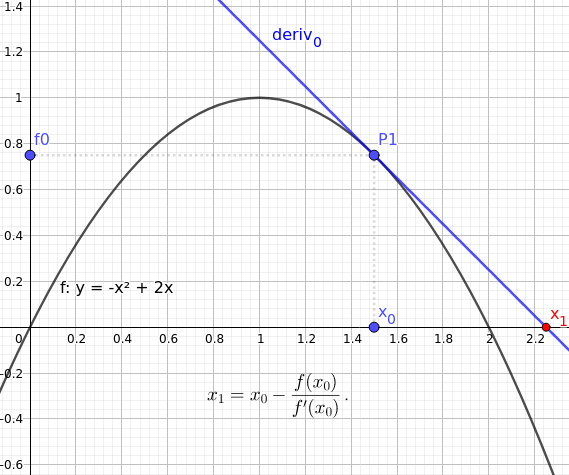
\includegraphics[width=0.55\textwidth]
      {src/MetodoNewton_grafico_1.png}
    \centering
    \caption{
      Primeira iteração do Método de Newton.
     }
    \label{MetodoNewton_grafico_1}
\end{figure}


E a partir do dado gráfico, agora podemos entender melhor como a iteração
funcionará, pois, o valor gerado, $x_1$, será aplicado no mesmo método. E com
isso, podemos construir a seguinte equação:

\begin{equation}
    x_{k+1} = x_{k} - \frac {f(x_{k})}{f'(x_{k})}.
    \label{newton_primeiraDeriv}
\end{equation}

Desse modo, gera-se uma sequência $\{x_k\}$, donde, esta, converge para a
raiz da função. E nesse sentido, vejamos a próxima iteração (Figura
\ref{MetodoNewton_grafico_2}) do exemplo mostrado na Figura
\ref{MetodoNewton_grafico_1}.

\begin{figure}[ht]
    \centering
    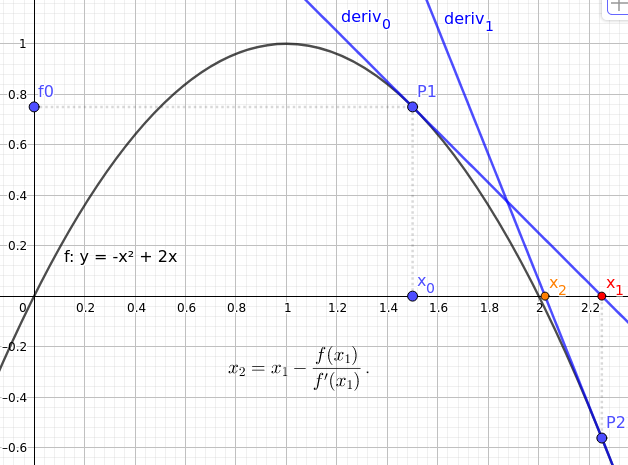
\includegraphics[width=0.55\textwidth]
      {src/MetodoNewton_grafico_2.png}
    \caption{
      Segunda iteração do Método de Newton.
    }
    \label{MetodoNewton_grafico_2}
\end{figure}

E assim, podemos notar a aproximação de $x_k$ para a raiz de $f$, observando o
ponto $x_2$.

Ademais, é válido ressaltar que o denominador da equação
\ref{newton_primeiraDeriv} tem que ser diferente de 0 (ou seja, a reta tangante
num ponto $P$ não pode ser paralela ao eixo x). No entanto, caso contrário,
isso significa que a dada função não possui raiz na proximidade daquele ponto.

\subsection{Encontrando Mínimos}

E é dessa maneira que, agora, podemos utilizar este método para encontrar
mínimos de uma função. Vimos que, o Método de Newton calcula raízes, e
desse modo, vinculando o que foi estudado no Capítulo 1, sabemos que, os
mínimos de uma função podem ser representados como raízes de sua derivada.

%TODO: Falar mais/melhor sobre a sequencia {x_k} (tendencia ao 0 da função)

Então, dado que as raízes de $f(x)$ podem ser geradas a partir da equação
\ref{newton_primeiraDeriv}, temos que: considerando $g(x)$ uma função duas vezes
derivável, e tendo como objetivo encontrar seus pontos de mínimo, pode-se
utilizar o Método de Newton para resolver tal problema da seguinte forma:

\begin{equation}
    x_{k+1} = x_{k} - \frac {g'(x_{k})}{g''(x_{k})}.
\end{equation}

Encontrando então as raízes aproximadas de sua derivada, e considerando
estas como  $x^*$, temos então que:

\begin{equation}
    g'(x^*) = 0.
\end{equation}

O método é simples, entrega muitas vezes ótimos locais próximos ao ponto
inicial, mas tem seu destaque, que é ser, facilmente computável.

Problemas de maximização podem ser vistos sob o seguinte olhar:

\begin{equation}
    max(f(x)) = min(-1 * f(x))
\end{equation}

Que com isto podem ser otimizados pelo Método de Newton também.

O movimento de \(x_k\) dentro da sequência, é determinado pela relação das
quantidades e propriedades, que tanto a primeira quanto a segunda derivada
oferecem. As quantidades, determinam a velocidade do movimento, e os sinais,
indicam a direção do movimento. De certa forma, podemos interpretar o movimento
da sequência \(\{x_k\}\) como instantes do movimento de uma bola numa ladeira,
que no começo de sua descida é acelerada, e, conforme chega ao plano no fim da
ladeira, começa a reduzir sua velocidade, até supostamente chegar no ponto mais
baixo.


\section{{Outros Métodos}}

Com o advento do Método de Newton, acabou surgindo uma família de métodos
similares. E como foi visto, é possível a partir dele, encontrar tanto raízes
de funções, quanto máximos/mínimos, herdando essa características para vários
dos métodos que o derivaram. São estes, Métodos Quasi-Newton e Método do
Gradiente Descendente, que, olhando como ponto de partida o Método de Newton, 
fornecem uma grande flexibilidade em como deseja-se utilizar os recursos de
precisão e poder computacional.

Métodos Quasi-Newton se fazem necessários quando nem sempre se tem acesso ou
recursos suficientes para se calcular a derivada de segunda ordem, ou até mesmo
a de primeira ordem. Já os métodos do Gradiente Descendente, como sugerido pelo
nome, utiliza-se majoritariamente da derivada de primeira ordem em seu processo.

Ademais, vejamos alguns outros métodos de otimização:

\subsection{Método do Gradiente Descendente}

Considerando que o Método de Newton encontra o \(min(f(x))\) através de uma
sequência \(\{x_k\}\):

\begin{equation}
    x_{k+1} = x_{k} - \frac {f'(x_{k})}{f''(x_{k})}.
\end{equation}

No qual, pode ser reescrito da seguinte forma:

\begin{equation}
    x_{k+1} = x_{k} -  \frac{1}{f''(x)} * f'(x_{k}).
\end{equation}

E, ressaltando que, sabemos que quem determina a direção da convergência é
\(f'(x)\), não é completamente necessário o uso de \( \frac{1}{f''(x)} \), que
tem como principal papel de controlar o tamanho do `passo dado' na iteração.
De modo que, a maioria dos Métodos Quasi-Newton fazem a substituição
da dada fração por aproximações boas o suficiente. E com isso, levando em
conta $\alpha$ como a representação dessa aproximação, temos:

\begin{equation}
    x_{k+1} = x_{k} -  \alpha * f'(x_{k}).
    \label{newton_lambda}
\end{equation}

Onde \(\alpha\) satisfaz:

\begin{equation}
    f(x_{k} -  \alpha * f'(x_{k})) < f(x_{x}).
    \label{newton_restricao_alpha}
\end{equation}

A partir da equação \ref{newton_lambda}, podemos escolher um \(\alpha\), de
modo que, seja menos custoso encontrá-lo do que calcular a segunda derivada
da função objetivo, ou até, podemos nem calculá-lo, basta considerar
um \(\alpha\) fixo, e tão pequeno que, quando a restrição
\ref{newton_restricao_alpha} não for cumprida, temos uma aproximação boa o
suficiente para o minimo da função.

Podemos assim dizer que esse modelo de resolução é útil e flexível o suficiente.
Tendo isso em mente, podemos seguir para o problema de encontrar o melhor
\(\alpha\), que já sabemos que sendo pequeno o suficiente minimiza a função, mas
talvez não da melhor forma possível. Sabemos que o \(\alpha\) tem que regular o
tamanho do passo. Ele pode ser usado em conjunto com outros elementos afim de
otimizar o processo de otimização.

Normalmente se é usado algum dos seguintes métodos para controlar o tamanho do
passo:

    \begin{itemize}
            \item Um valor fixado para \(\alpha\);
            \item Um método que atualize \(\alpha\) de acordo com alguma situação;
            \item Um método que escolha um valor ótimo ou quase ótimo para \(\alpha\);
            \item Um elemento que forneça mais informações sobre a função trabalhando em conjunto com o \(\alpha\).
    \end{itemize}


Simplesmente considerar um \(\alpha\) um valor fixo e pequeno pode funcionar,
mas não seguramente para qualquer situação, como por exemplo uma função que
possui "movimentos bruscos" em um escala minuscula, ou ainda, caso se tenha
considerado um ponto inicial muito distante de qualquer ótimo que seja, o que
faz com que o algoritmo seja absurdamente custoso.

Atualizar o valor de \(\alpha\) de acordo com a situação do processo iterativo
de otimização pode ser uma boa opção quando não se tem tanto pode computacional.
Comumente pode ser encontrado implementações que iniciam com um \(\alpha\) não
tão pequeno (isso ajuda a resolver o problema de iniciar com um ponto longe da 
solução), mas ao passar das iterações, reduzir o seu valor por algum fator.
Fator este que pode ser alguma relação com a magnitude da derivada, já que ela
pode nos dar uma dica do quão longe o ótimo está do ponto atual, ou ainda
considerar o fator de redução como a relação com a iteração atual:


Considerando \(\alpha_{0} \in \mathbb{R}^{+}  \), e \(k\) a k-ésima iteração:

\begin{equation}
    \alpha_{k+1} = \frac{\alpha_{k}}{k}
\end{equation}

Ou ainda:

\begin{equation}
    \alpha_{k+1} = \frac{\alpha_{k}}{2} = \frac{\alpha_{0}}{2^k} 
\end{equation}


Quando começamos a observar outras formas de melhorar o valor de \(\alpha\),
acabamos por entrar em uma recursão, pois dai começa todo um estudo sobre como
otimizar um parâmetro específico de um otimizador. Os métodos mais famosos que
buscam valores ótimos ou quase ótimos para \(\alpha\) são os métodos
\textit{line search}. Os quais normalmente se trabalham com condições específicas
sobre a otimalidade de \(\alpha\), como as condições de Wolfe por exemplo. Tais
métodos utilizam-se dos artifícios citados anteriormente, já que são uma peça
básica na construção do otimizador, ou ainda podem se utilizar de métodos fora
dessa família de métodos newtonianos.

Agora, antes de seguirmos para a analise de algum elemento de ajuda no valor, se
faz necessária uma nova observação sobre a estrutura básica dos métodos. Até o
momento viemos considerando apenas a derivada de primeira ordem como sendo a
direção certa a ser tomada. Vamos tomar a seguinte equação:

\begin{equation}
    x_{k+1} = x_{k} - \alpha * \frac{1}{f''(x_k)} * f'(x_k)
\end{equation}

Se tomarmos \(\alpha = 1\) temos o método em sua forma natural. Mas ainda
podemos procurar um valor para \(\alpha\) que melhore ainda mais a iteração.
E mais, sabemos sobre as acusações que as derivadas de segunda ordem fazem,
sobre a otimalidade, sendo assim podemos dizer que a direção de otimização,
na verdade, é dada por:

\begin{equation}
    p_k = \beta(x_k) * f'(x_k)
\end{equation}

Então:

\begin{equation}
    x_{k+1} = x_{k} - \alpha * p_{k}
\end{equation}


Dai temos normalmente 3 opções no que se diz respeito ao \(\beta(x_k)\):

A primeira é considerar \(\beta(x_k) \frac{1}{f''(x_k)}\), o que nos dá
o método de Newton, novamente, e o \(\alpha\) não passaria de um mero ajuste.

A segunda opção é considerar \(\beta(x_k) \approx \frac{1}{f''(x_k)}\), o que
abre um leque de possibilidade no que diz respeito ao calculo dessa aproximação,
e, tornando-se assim um método Quasi-Newton. Esse formato é um dos mais
populares, sendo os métodos de otimização padrões em bibliotecas cientificas,
como scipy em Python, e GSL em C. Sendo um dos mais famosos o método BFGS
(Broyden-Fletcher-Goldfarb-Shanno).


A terceira opção é considerar \(\beta(x_k) \) neutro, de forma que:
\begin{equation}
    p_k = \beta(x_k) * f'(x_k) = f'(x_k)
\end{equation}

Assim tendo um método do Gradiente Descendente, que como dito anteriormente,
normalmente é resolvido por um método de \textit{line search}.






\subsection{Simplex}

\hspace{0.8cm}
O método Simplex, pode ser classificado como clássico, por ser um
dos métodos mais famosos. Formulado por George B. Dantzig, fruto de uma
sugestão de outro homem, T. S. Motzkin, que contribuiu para diversas áreas da
matemática.

Os problemas que o método Simplex resolve, fazem parte de uma conjunto de
problemas de Otimização Linear (ou Programação Linear), os quais se restringem
a, apenas, funções lineares. Além disso, tais problemas normalmente acompanham
restrições, sobre as entradas da função a ser otimizada.

Um problema de otimização linear, pode ser resumido em:

\begin{equation}
        Z = c_1x_1 + c_2x_2 + … + c_nx_n
\end{equation}

E tendo restrições também lineares para a função objetivo, como:
\begin{equation}
    \begin{split}
        &   a_{11}x_1 + a_{12}x_2 + … + a_{1n}x_n \leq b_1\\
        &   a_{21}x_1 + a_{22}x_2 + … + a_{2n}x_n \leq b_2\\
        &   ...\\
        &   a_{m1}x_1 + a_{m2}x_2 + … + a_{mn}x_n \leq b_m\\
        &   x_1 \geq 0, x_2 \geq 0, …, x_n \geq 0
    \end{split}
\end{equation}

O tipo de problema que o Simplex resolve, se desenvolve como a seguir:

\begin{equation}
        max \{c^tx | Ax \leq b, x \geq 0\}\\
\end{equation}


A forma de operação desse método é semelhante ao que uma pessoa comumente faria
ao se deparasse com o problema de forma gráfica. O problema, sendo
completamente linear, gera retas, que acabam por formando regiões de
possíveis soluções, e dessas regiões, queremos saber qual a melhor solução.
Para isso, bastaria procurar dentro de tal região, onde o valor da função Z é o
maior possível. Uma vez a região sendo construída por retas, acaba por
ter a característica de ser convexa, como um polígono convexo no plano ou um
poliedro convexo no espaço, o que a acaba por facilitar a busca pelo máximo,
dentro dessa região, uma vez que basta olha os vértices de tal região.

Repara-se, que, o método Simplex não se utiliza de artifícios e ferramentas do
Cálculo, como nos métodos anteriormente apresentados, mas sim, formas
diferentes de analisar o problema, que por certos aspectos é simples. O método
completo é constituído por operações em uma matriz específica (Tableau), que
representa o problema, o qual não é necessário ser apresentado aqui, por se
distanciar da `família' de métodos de otimização que é apresentado neste
documento.



\section{{Programando os Métodos}}

\hspace{0.8cm}

\subsection{Método de Newton}

\hspace{0.8cm}
A forma mais simples e mais útil de implementar o Método de Newton, é na forma
de busca das raízes, que, uma vez implementada, só precisamos por como entrada
a primeira e a segunda derivada da função que desejamos minimizar, já que o
método não precisa saber qual a função de fato. A seguir temos a implementação
na linguagem de programação \textit{Rust}:
\vspace{0.2cm}
\begin{lstlisting}
pub fn newton1x1<F>(funcao_derivada: &F, x: f64) -> (usize, f64)
where
    F: Fn(f64) -> f64,
{
    let mut entrada_atual = x;
    let maximo_iteracoes = 100;

    for iteracao_atual in 1..=maximo_iteracoes {
        let diferenca: f64 =
            funcao_derivada(entrada_atual.clone())
            /
            derive1x1(&funcao_derivada, &entrada_atual);

        println!("diferenca: {}", diferenca);
        entrada_atual -= diferenca;

        if diferenca.abs() < 0.0000001 {
            return (iteracao_atual, entrada_atual);
        }
    }

    return (maximo_iteracoes, entrada_atual);
}
\end{lstlisting}


Os parâmetros da função são:

    \begin{itemize}
            \item Uma função \(f : \mathbb{R} \rightarrow \mathbb{R}\)
            \item Uma entrada x sendo o chute inicial do ótimo.
    \end{itemize}


A função \textit{derive1x1}, recebe como parâmetro uma função e um ponto,
tendo como retorno, a derivada da função entregue, no ponto especificado.
Restringindo-se à funções do tipo \(f : \mathbb{R} \rightarrow \mathbb{R}\).


\subsection{Método do Gradiente Descendente}

\hspace{0.8cm}
A implementação desse método, exige apenas, que seja definido o cálculo
da derivada da função objetivo, o valor de $\alpha$, um palpite inicial para
o valor de x, e a quantidade de iterações desejada. Também, pode ser
indicado um valor que se refere a diferença dos dois últimos valores
da sequência \{$x_k$\}, podendo assim, efetuar a parada da execução do
método. A seguir, temos a implementação na linguagem de programação
\textit{C++}:

\vspace{0.2cm}
\begin{lstlisting}[language=C++]

// Sendo f(x) = x^4 - 3*x^3 + 2
#include <bits/stdc++.h>
#define decimal long double
using namespace std;
// Calcula a derivada da funcao
decimal df(decimal x) {
	return 4 * pow(x, 3) - 9 * pow(x, 2);
}
int main() {
	// Palpite inicial
	decimal x_proximo = 5.5;
	// Variavel para iterar
	decimal x_atual;
	// Quantidade maxima de iteracoes
	int iteracoes = 100000;
	decimal alpha = 0.00001;
	// Precisao para condicao de parada
	decimal precisao = 0.000000001;
	// Comeca as iteracoes
	while(iteracoes > 0) {
		x_atual = x_proximo;
		x_proximo = x_atual - (alpha * df(x_atual));
		decimal precisao_atual = x_atual - x_proximo;
		// Se atingir a precisao desejada
		if(abs(precisao_atual) < precisao)
			break; // Para as iteracoes
		// Conclui uma iteracao
		iteracoes -= 1;
	}
	cout << ``x que minimiza f(x) = '' << x_proximo << endl;
	// Saida do algoritmo:
	// --> x que minimiza f(x) = 2.25
	return 0;
}


\end{lstlisting}





textcolor[rgb]{1,0,0}{\section{{O Método de Newton para Várias Variáveis}}}

%%%%%%%%%%%%%%%%%%%%%%%%%%%%%%%%%%%%%%%%%%%%%%%%%
% Relatório Final - Projeto de Pesquisa
% Métodos de Otimização
% Baltz & Machado
% Capítulo 3
%%%%%%%%%%%%%%%%%%%%%%%%%%%%%%%%%%%%%%%%%%%%%%%%%


\chapter{\Large{Os Métodos Modernos de Otimização}} \label{chp:3}


\section{Breve Relato Histórico}

\hspace{0.8cm}

\section{{Métodos de Um}}

\hspace{0.8cm}

\subsection{O Método - Uma breve descrição}

\subsection{Exemplos Aplicações}

\subsection{Possíveis Aplicações}


\section{{Métodos de Dois}}

\hspace{0.8cm}

\subsection{O Método - Uma breve descrição}

\subsection{Exemplos Aplicações}

\subsection{Possíveis Aplicações}

\textcolor[rgb]{1,0,0}{\section{{Um com o outro}}}

%%%%%%%%%%%%%%%%%%%%%%%%%%%%%%%%%%%%%%%%%%%%%%%%%
% Relatório Final - Projeto de Pesquisa
%Métodos de Otimização
% Baltz & Machado
% Capítulo 4
%%%%%%%%%%%%%%%%%%%%%%%%%%%%%%%%%%%%%%%%%%%%%%%%%


\chapter{\Large{Aplicações à Mecânica Celeste}} \label{chp:4}


\section{Entendendo o Problema de N Corpos}


\section{{A Otimização na Mecânica}}


\section{Resultados Numéricos}




%%%%%%%%%%%%%%%%%%%%%%%%%%%%%%%%%%%%%%%%%%%%%%%%%
% Relatório Final - Projeto de Pesquisa
% Métodos de Otimização
% Baltz & Machado
% Capítulo 5
%%%%%%%%%%%%%%%%%%%%%%%%%%%%%%%%%%%%%%%%%%%%%%%%%


\chapter{\Large{Demais Resultados}}\label{chp:5}


\section{{Outros Resultados}}


\subsection{{}}

%%%%%%%%%%%%%%%%%%%%%%%%%%%%%%%%%%%%%%%%%%%%%%%%%
% Relatorio Final - Métodos de Otimização
% Referências Bibliográficas
% Baltz & Machado
%%%%%%%%%%%%%%%%%%%%%%%%%%%%%%%%%%%%%%%%%%%%%%%%%

\begin{thebibliography}{99}

\addcontentsline{toc}{chapter}{\normalsize Bibliografia}

       \bibitem {AppliedOptimization} \textit{Liqun Qi, Kok Lay Teo, Xiao Qi Yang.} {\it Applied Optimization}. \textit{Springer, Optimization and control with applications. 2005.}
       % \bibitem {algebralinear} \textit{Lima, Elon Lajes} {\it Álgebra Linear}. \textit{7º Edição. Rio de Janeiro; IMPA, 2008.}
       % \bibitem {algebralinear1} \textit{Halmos, Paul R.} {\it Espaços Vetoriais de Dimensão Finita}. \textit{Tradução [de] Guilherme de la Penha. Rio de Janeiro: Campus, 1978.}


       \end{thebibliography}


\end{document}
